By the Hillas cryterion,
\begin{equation}
  E_\text{max} \approx 2 \beta c Z e B r.
\end{equation}

With $r=\SI{4}{\kilo\meter}$, $B=\SI{10}{\tesla}$, $Z=1$, and the particles traveling at nearly the speed of light ($\beta\rightarrow 1$),
\begin{align}
  E_\text{max} \approx 2
    \times \SI{3e8}{\meter\per\second}
    \times 1
    \times \SI{1.602e-19}{\coulomb}
    \times \SI{10}{\tesla}
    \times \SI{4}{\kilo\meter}
  \approx \boxed{ \SI{24}{\tera\electronvolt} }
\end{align}

This places LHC below the theoretical cutoff line on the Hillas diagram, corresponding to $\sim\!10^{20}\eV$. The LHC's magnetic field and size are about 7 orders of magnitude smaller than
the CR sources at the theoretical cutoff.
\begin{figure}[H]
  \centering
  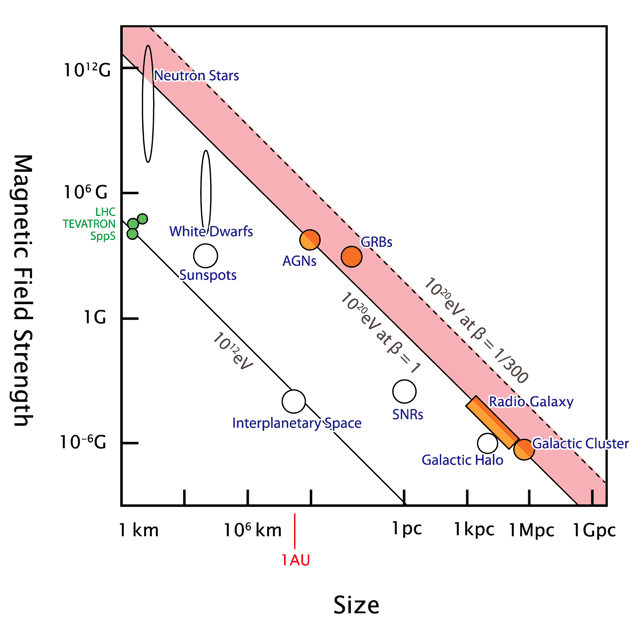
\includegraphics[width=0.6\linewidth]{hillas_diagram}
  \put(-120,25){\small Figure from}
  \put(-120,10){\small \url{http://jemeuso.riken.jp/en/about2.html}}
\end{figure}


To accelerate particles to $E=\SI{1}{\zetta\electronvolt}=\SI{1e21}{\electronvolt}$, an accelerator of this size would need a magnetic field of
\begin{equation}
  B_2 = \frac{E_2}{E_1} \times B_1
      = \frac{\SI{1e21}{\electronvolt}}{\SI{24e12}{\electronvolt}} \times \SI{10}{\tesla}
      = \boxed{ \SI{4.16e9}{\tesla} }
\end{equation}

The maximum energy of an accelerator circling the earth ($r=\SI{6.4e6}{\meter}$) with a $\SI{10}{\tesla}$ field would be
\begin{equation}
  E_3 = \frac{r_3}{r_1} \times E_1
      = \frac{\SI{6.4e6}{\meter}}{\SI{4e3}{\meter}} \times \SI{24e12}{\electronvolt}
      = \boxed{ \SI{3.84e4}{\tera\electronvolt} }
\end{equation}

